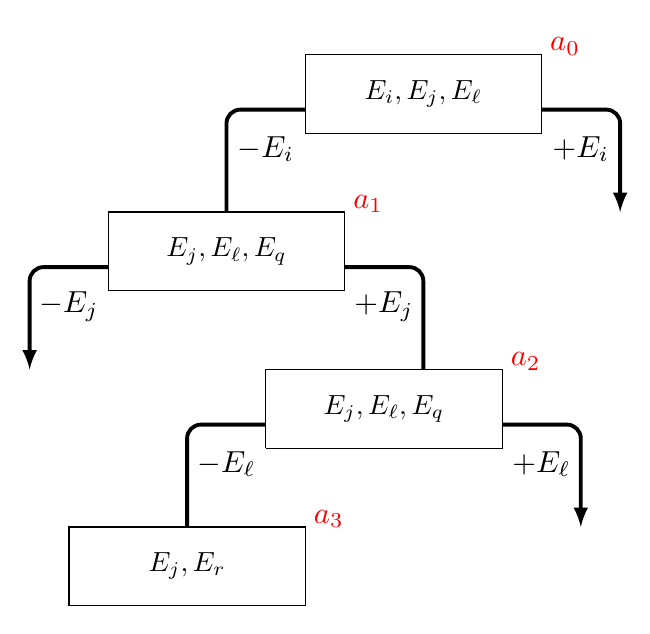
\begin{tikzpicture}

% BLOCS %%%%%%%%%%%%%%%%%%%%%%%%%%%%%%%%%%%%%%%%%%%%%%%%%%%%%%%%%%%%%%%%%%

\draw [color = black, fill = white] (6.0,10.0) -- (6.0,11.0) -- (9.0,11.0) -- (9.0,10.0) --  (6.0,10.0);
\draw [color = black, fill = white] (3.5,8.0) -- (3.5,9.0) -- (6.5,9.0) -- (6.5,8.0) -- (3.5,8.0);
\draw [color = black, fill = white] (5.5,6.0) -- (5.5,7.0) -- (8.5,7.0) -- (8.5,6.0) -- (5.5,6.0);
\draw [color = black, fill = white] (3.0,4.0) -- (3.0,5.0) -- (6.0,5.0) -- (6.0,4.0) -- (3.0,4.0);

% CUBES

\node (P1) at (7.5,10.5) {$\set{E_i,E_j,E_{\ell}}$};
\node (P2) at (5.0,8.5) {$\set{E_j,E_{\ell},E_q}$};
\node (P3) at (7.0,6.5) {$\set{E_j,E_{\ell},E_q}$};
\node (P4) at (4.5,4.5) {$\set{E_j,E_r}$};


% ETIQUETTES


\node[scale=1.1, color = red] at (9.3,11.1) {$a_0$};
\node[scale=1.1, color = red] at (6.8,9.1) {$a_1$};
\node[scale=1.1, color = red] at (8.8,7.1) {$a_2$};
\node[scale=1.1, color = red] at (6.3,5.1) {$a_3$};

\node[scale=1.1] at (5.5,9.8) {$-E_i$};
\node[scale=1.1] at (9.5,9.8) {$+E_i$};

\node[scale=1.1] at (3.0,7.8) {$-E_j$};
\node[scale=1.1] at (7.0,7.8) {$+E_j$};

\node[scale=1.1] at (9.0,5.8) {$+E_{\ell}$};
\node[scale=1.1] at (5.0,5.8) {$-E_{\ell}$};


% LINKS %%%%%%%%%%%%%%%%%%%%%%%%%%%%%%%%%%%%%%%%%%%%%%%%%%%%%%%%%%%%%%%%%%
%\draw[line width = 2pt, color=blue, dashed] (10.5,10.5)--(12.8,10.5);
%\draw[line width = 2pt, color=blue, dashed] (7.5,8.0)--(12.8,8.0);
%\draw[line width = 2pt, color=blue, dashed] (5.5,5.5)--(12.8,5.5);
%\draw[->,>=latex,line width = 2pt, color=blue] (13.2,12.0)--(13.2,4.0);

\draw[rounded corners=5pt,line width = 1.4pt] (6.0,10.3) -| (5.0,9.0);
\draw[->,>=latex,rounded corners=5pt,line width = 1.4pt] (3.5,8.3) -| (2.5,7.0);

\draw[->,>=latex,rounded corners=5pt,line width = 1.4pt] (9.0,10.3) -| (10.0,9.0);

%\draw[->,>=latex,line width = 1.4pt] (5.5,7.5) -- (5.5,6.0);
\draw[rounded corners=5pt,line width = 1.4pt] (6.5,8.3) -| (7.5,7.0);

\draw[rounded corners=5pt,line width = 1.4pt] (5.5,6.3) -| (4.5,5.0);
\draw[->,>=latex,rounded corners=5pt,line width = 1.4pt] (8.5,6.3) -| (9.5,5.0);


\end{tikzpicture}
